\section{Theorie}
Der Faraday-Effekt oder auch die Faraday-Rotation, beschreibt die Drehung der
Polarisationsebene eines Lichtstrahls beim Durchlaufen von Materie unter dem
Einfluss eines Magnetfeldes. Mit Hilfe des Effektes ist es möglich die
Bandstruktur in einem Halbleiter zu verstehen und die effektive Elektronenmasse
in diesem zu bestimmen.

\subsection{Das quantenmechanische Bändermodell}
Das quantenmechanische Bändermodell beschreibt das Energiespektrum eines
Elektrons in einem Kristall. Ein einzelnes Atom besitzt ein diskretes
Energiespektrum. Werden zwei Atome angenähert, sodass sie miteinander
wechselwirken, werdend die einzelnen Energieniveaus breiter. In einem Kristall
wechselwirken eine Mehrzahl von Atomen, sodass die Energieniveaus zu breiten
Bändern werden. Das Bändermodell eines Halbleiters wird in Abbildung
\ref{fig:band} dargestellt.

\begin{figure}[H]
  \centering
  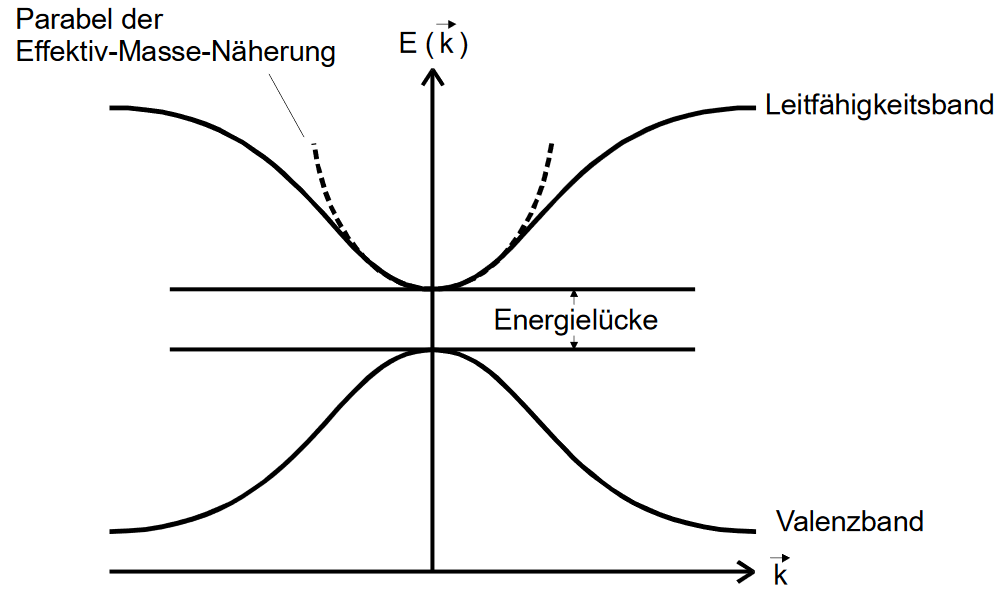
\includegraphics[width=13cm, height=7cm]{bandmodel.png}
  \caption{Vereinfachtes Bändermodell für einen Festkörper}
  \label{fig:band}
  \cite{skript}
\end{figure}

In dieser Abbildung werden die drei wichtigen Bereiche in einem Festkörper
dargestellt. Das Valenzband ist komplett mit Elektronen besetzt und trägt nicht
zur Leitfähigkeit eines Körpers bei. Das Leifähigkeitsband ist nicht
vollständig besetzt und ist somit für die Leitfähigkeit eines Festkörpers von
Bedeutung. Zwischen diesen Bereichen befindet sich eine Energielücke. Besitzt
die Energielücke eine Breite von über $\SI{10}{\electronvolt}$, so können die
Elektronen aus dem Valenzband selbst mit hinzugefügter Energie diese Lücke nicht
überwinden, der Körper ist somit ein Nichtleiter. Überlappen sich die beiden
Bänder, so wird der Festkörper als Leiterbezeichnet. Halbleiter besitzten eine
Energielücke, die die Elektronen nach hinzugefügter Energie noch überwinden
können. Daher stammt auch der Begriff des Halbleiters. Erst nachdem eine
gewisse Energie beispielsweise in Form von Wärme hinzugefügt wird, können die
Elektronen die Lücke überwinden und der Körper leitet. Wird keine Energie
hinzugefügt, befinden sich die Elektronen im Valenzband in einer festen Bindung
und können die Lücke nicht überwinden, der Stoff ist somit nicht leitend. Die
Elektronenenergie in Abhängigkeit vom Wellenzahlvektor ist gegeben durch die
Beziehung
\begin{equation}
  \epsilon = \frac{\hbar^2 \text{k}^2}{2 \text{m}}
\end{equation}

\subsection{Die effektive Masse}
Da von kugelflächigen Energieflächen ausgegangen werden kann, ergibt sich nach
einer Näherung durch Taylor folgende Funktion für die Elektronenenergie
\begin{equation}
  \epsilon\left(\vec{\text{k}}\right) = \epsilon(0) + \frac{\hbar^2 \text{k}^2}
  {2 \text{m}^*}
  \label{eqn:sgl}
\end{equation}
Dabei beschreibt $\text{m}^*$ die effektive Masse. Die Energiewerte aus
Gleichung \eqref{eqn:sgl} beschreiben die Lösungen der Schrödinger-Gleichung
für ein freies Elektron. Die Verwendung der effektiven Masse ist aus mehreren
Gründen sinnvoll. Einerseits berücksichtigt die effektive Masse das
Kristallpotential. Außerdem können Elektronen in einem Band durch die effektive
Masse wie freie Teilchen berechnet werden. Mathematisch wird es somit auf ein
bekanntes und lösbares Problem zurückgeführt von welchem auf die eigentliche
Masse zurückgeschlossen werden kann.

\subsection{Die zirkuläre Doppelbrechung}
Zwei wichtige Arten der Polarisation sind zu einem lineare und zu anderem
zirkulär Polarisation. Bei der linearen Polarisation schwingt die Welle
senkrecht zur Ausbreitungsrichtung. Sie findet somit in einer Ebene statt.
Zirkulär polarisiertes Licht rotiert jedoch um die Achse der
Ausbreitungsrichtung. Linear Polarisiertes Licht kann durch eine Zusammensetzung
von links und rechts polarisiertem Licht beschrieben werden.
Tritt eine linear polarisierte Welle in einem Kristall wird die
Polarisationsebene des Lichtstrahls auf Grund der veschiedenen
Phasengeschiwindigkeiten der zirkulären Komponenten gedreht.
Beim eintritt der Welle in den Kristall bei einer Ausbreitung in $z$-Richtung
besitzt die Welle lediglich eine $x$-Komponente. Nach Durchlaufen des Kristalls
weist die Welle jedoch eine zusätzliche $y$-Komponente auf. Die Welle wird somit
um den Winkel $\theta$ gedreht. Da sich der Brechungsindex mit Hilfe der
Phasengeschwindigkeit berechnen lässt, existieren auch zwei Brechungsindizes.
Die Drehung wird auch zirkulären Doppelbrechung genannt und wird in
Abbildung \ref{fig:rotation} dargestellt.

\begin{figure}[H]
  \centering
  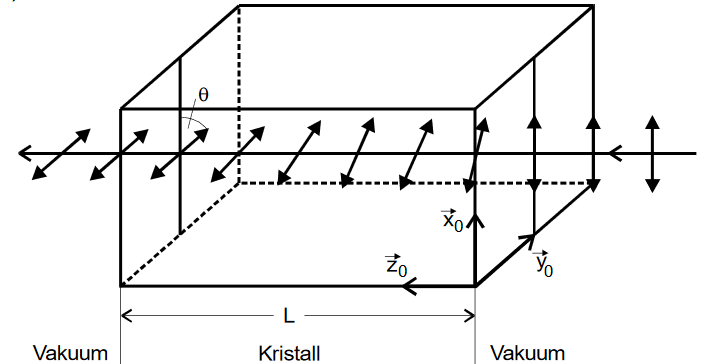
\includegraphics[width=12cm, height=6cm]{rotation.png}
  \caption{Zirkuläre Doppelbrechung in einem Kristall}
  \label{fig:rotation}
  \cite{skript}
\end{figure}


Die Doppelbrechung entsteht durch elektrische Dipolmomente der Atome auf den
Gitterplätzen und durch die Wechselwirkung der Bandelektronen mit den Rümpfen der
Atome. Die Anzahl der Dipolmomente pro Volumeneinheit erzeugt die Polarisation
des Kristalls.

\subsubsection{Die dielektrische Suszeptibilität}
\label{sssec:sus}
Die Proportionalitätskonstante zwischen Polarisation $\vec{\text{P}}$ und dem
elektrischen Feld $\vec{\text{E}}$ wird dielektische Suszeptibilität $\chi$
genannt. Diese Größe ist in diesem Fall ein Tensor, da es sich um anisotrope,
also richtungsabhängige, Kristalle handelt. Sobald ein Material doppelbrechend
ist, besitzt der Tensor neben den Einträgen auf der Hauptdiagonalen zwei
komplex konjugierte, nicht diagonale Einträge. Das führt dazu, dass die
Phasengeschwindigkeit für links oder rechts zirkuläres Licht entweder größer
oder kleiner ist als die Phasengeschwindigkeit für einen Tensor ohne Elemente
außerhalb der Hauptdiagonalen.

\subsection{Der Faraday-Effekt für optisch inaktive Materie}
Der Faraday-Effekt, also die Drehung der Polarisationsebene eines Lichtstrahls
beim Eintritt in einen Kristall, ist nicht nur bei Materialien mit dem in
Kapitel \ref{sssec:sus} beschriebenen Tensor möglich. Unter Einfluss eines
Magnetfeldes ist dieser Effekt auch bei Materie mit einem Tensor, der
lediglich Einträge auf der Hauptebene besitzt, möglich. Unter Einfluss eines
Magnetfeldes ändert sich die zu Beginn isotrope, also richtungunabhängige, Masse
jedoch und bekommt komplex konjugierte Einträge auf der nicht diagonalen. Die
Materie ist somit doppelbrechend geworden. Das bedeutet, dass ein Magnetfeld
einfluss auf die Symmetrie eines Kristalles hat. Der Winkel $\theta$ ist dann
proportional zur Flussdichte $\text{B}$, der Länge des Kristalls $\text{L}$ und
zur Zahl der Ladungsträger pro Volumeneinheit $\text{N}$. Die
Frequenzabhängigkeit lässt sich mit Hilfe der Zyklotron-Frequenz $\omega_0$
beschreiben. Die Zyklotron-Frequenz beschreibt die Umlauffrequenz von Elektronen,
die unter Einfluss der Lorentz-Kraft eine Kreisbahn umlaufen. 
